
\begin{frame}
    \begin{center}
        \LARGE 江门中微子实验探测器模拟及离线软件
    \end{center}
\end{frame}

\begin{frame}
    \frametitle{江门中微子实验软件工作}
    \begin{itemize}
        \item 离线软件环境的维护。
        \item 探测器模拟软件的开发。
        \item 几种不同方案探测器的模拟。
            \begin{itemize}
                \item 能量分辨率的研究,
                \item 放射性本底对能量分辨率的影响。
            \end{itemize}
        \item 基于Sniper离线框架的探测器模拟软件。
    \end{itemize}
\end{frame}

\begin{frame}
    \frametitle{离线软件环境的维护}
    \begin{itemize}
        \item 外部库的重新安装(由于panfs盘的下线)。
            \begin{itemize}
                \item 目前迁移至{\tt
                    /afs/ihep.ac.cn/soft/dayabay/jmne/external/local}
                \item 图形库Qt的安装。目前编译的Geant4使用Qt作为UI。
            \end{itemize}
        \item 完善了geant4中使用的数据集(
              原先的geant4没有安装完整的数据集,导致看不到放射性衰变)。
        \item 由于离线软件将使用subversion进行版本控制,
              因此配置了svn服务器。并使用Trac对svn进行用户授权。
        \item 原先的探测器模拟程序目前仍旧使用git进行版本控制。
    \end{itemize}
\end{frame}

\begin{frame}
    \frametitle{使用Trac对svn进行用户及权限管理}
    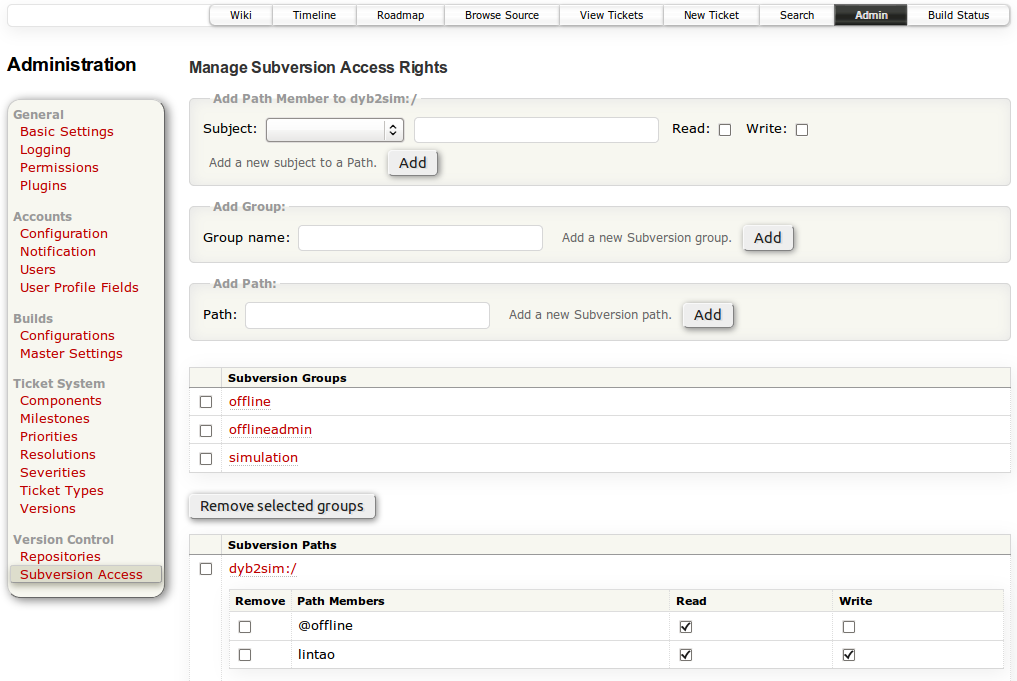
\includegraphics[width=12cm,keepaspectratio]{data/trac_svn.png}
\end{frame}

\begin{frame}
    \frametitle{模拟软件的开发}
    \begin{itemize}
        \item 产生子
            \begin{itemize}
                \item 支持按照时间将HepEvt事例拆分成子事例
                \item 支持GENIE中产生的RooTracker格式(加速器中微子)
            \end{itemize}
        \item 物理过程
            \begin{itemize}
                \item 修正了Optical Rayleigh Scattering的bug。
                      (由于大亚湾一期的Rayleigh Scattering是基于Geant4 9.2,
                       而到9.4中这个bug才修复。)
                       \footnote{由北大王思广指出}
                \item 添加了中子俘获散射截面及末态信息数据。
                      (一期中使用了NNDC核数据库的数据,
                      而在我们初期的模拟中,我们没有注意到要使用这些数据。)
                       \footnote{由山大陈泉佑指出}
                \item 对旧式的低能电磁过程及新式的Livermore模型进行比较。
            \end{itemize}
        \item PMT相关的研究
            \begin{itemize}
                \item 对PMT几何进行了研究。初步了解TorusStack的构建方法。
                \item 修正20英寸Torus Stack的问题。
                      \footnote{由武大丁雪峰指出}
                \item 尝试对PMT的构造进行改造(未完成,仍有overlap的问题)。
            \end{itemize}
    \end{itemize}
\end{frame}

\begin{frame}
    \frametitle{不同构造方式的PMT}
    \begin{columns}
        \column{6.0cm}
        \begin{figure}
            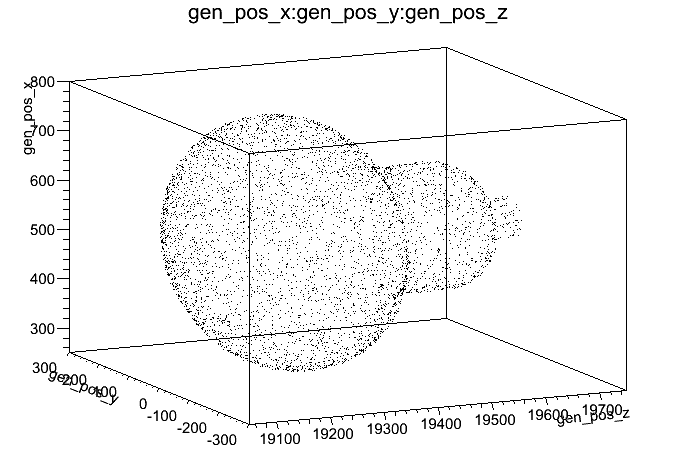
\includegraphics[width=6cm,keepaspectratio]{data/torusstack_PMT.png}
            \caption{Torus Stack方式构建}
        \end{figure}
        \column{6.0cm}
        \begin{figure}
            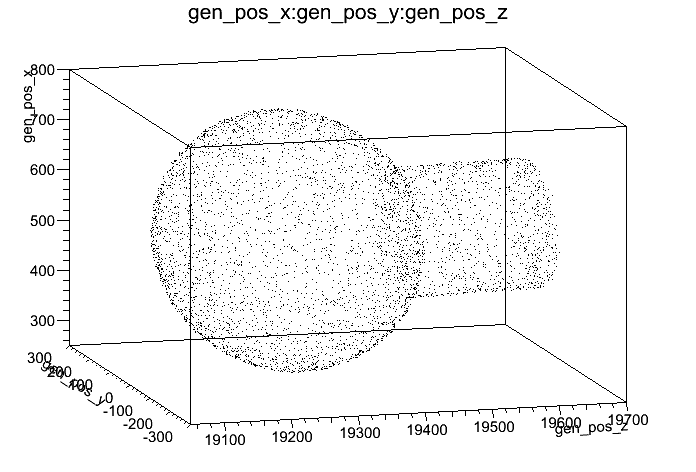
\includegraphics[width=6cm,keepaspectratio]{data/ellipsoid_PMT.png}
            \caption{Ellipsoid方式构建}
        \end{figure}
    \end{columns}
\end{frame}


\begin{frame}
    \frametitle{不同方案探测器的模拟}
    \begin{itemize}
        \item
    \end{itemize}
\end{frame}

\newsavebox{\NoviceJobOptions}
\begin{lrbox}{\NoviceJobOptions}
\begin{lstlisting}[language=c++]
#include "$DETSIMROOT/share/jobOptions.txt"
Sniper.Dlls += {"Novice01"};
SvcMgr.Contents += {"ExN01Factory"};

Sniper.Cycler = "NormCycler";
Sniper.InputSvc = "NONE";

DetSim.DetFactory = "ExN01Factory";
DetSim.RunMac = "run.mac";

Sniper.EvtMax   = 2;
Sniper.LogLevel = 3; // INFO
\end{lstlisting}
\end{lrbox}


\begin{frame}
    \frametitle{基于Sniper离线框架的模拟}
    \begin{itemize}
        \item Sniper是新的软件框架,追求简洁,适合非对撞实验。
        \item 主要提供了算法,服务和工具。
        \item 参考邓子艳老师的工作,对Geant4中{\tt RunManager}进行了改造。
              使其更适合于Sniper这个框架。
        \item 为了使原有的geant4程序修改最小,需要额外提供一个抽象工厂,
              这样基于Sniper的DetSim会根据此工厂自动构建探测器。
    \end{itemize}
    \par\usebox{\NoviceJobOptions}
\end{frame}

\newsavebox{\NoviceHeader}
\begin{lrbox}{\NoviceHeader}
\begin{lstlisting}[language=c++]
class ExN01Factory:  virtual public SvcBase , 
                     virtual public IDetSimFactory {
public:
    ExN01Factory(const std::string& name);
    virtual ~ExN01Factory();

    virtual G4VUserDetectorConstruction* createDetectorConstruction();
    virtual G4VUserPhysicsList* createPhysicsList();
    virtual G4VUserPrimaryGeneratorAction* createPrimaryGenerator();

    virtual bool initialize();
    virtual bool finalize();
};
\end{lstlisting}
\end{lrbox}

\begin{frame}
    \frametitle{Novice 01 需要提供的抽象工厂:头文件}
    \par\usebox{\NoviceHeader}
\end{frame}

\newsavebox{\NoviceImpl}
\begin{lrbox}{\NoviceImpl}
\begin{lstlisting}
G4VUserDetectorConstruction*
ExN01Factory::createDetectorConstruction()
{   
    return new ExN01DetectorConstruction;
}

G4VUserPhysicsList*
ExN01Factory::createPhysicsList()
{   
    return new ExN01PhysicsList;
}

G4VUserPrimaryGeneratorAction*
ExN01Factory::createPrimaryGenerator()
{   
    return new ExN01PrimaryGeneratorAction;
}
\end{lstlisting}
\end{lrbox}

\begin{frame}
    \frametitle{Novice 01 需要提供的抽象工厂:实现}
    \par\usebox{\NoviceImpl}
\end{frame}

